% Options for packages loaded elsewhere
\PassOptionsToPackage{unicode}{hyperref}
\PassOptionsToPackage{hyphens}{url}
%
\documentclass[
]{article}
\usepackage{lmodern}
\usepackage{amsmath}
\usepackage{ifxetex,ifluatex}
\ifnum 0\ifxetex 1\fi\ifluatex 1\fi=0 % if pdftex
  \usepackage[T1]{fontenc}
  \usepackage[utf8]{inputenc}
  \usepackage{textcomp} % provide euro and other symbols
  \usepackage{amssymb}
\else % if luatex or xetex
  \usepackage{unicode-math}
  \defaultfontfeatures{Scale=MatchLowercase}
  \defaultfontfeatures[\rmfamily]{Ligatures=TeX,Scale=1}
\fi
% Use upquote if available, for straight quotes in verbatim environments
\IfFileExists{upquote.sty}{\usepackage{upquote}}{}
\IfFileExists{microtype.sty}{% use microtype if available
  \usepackage[]{microtype}
  \UseMicrotypeSet[protrusion]{basicmath} % disable protrusion for tt fonts
}{}
\makeatletter
\@ifundefined{KOMAClassName}{% if non-KOMA class
  \IfFileExists{parskip.sty}{%
    \usepackage{parskip}
  }{% else
    \setlength{\parindent}{0pt}
    \setlength{\parskip}{6pt plus 2pt minus 1pt}}
}{% if KOMA class
  \KOMAoptions{parskip=half}}
\makeatother
\usepackage{xcolor}
\IfFileExists{xurl.sty}{\usepackage{xurl}}{} % add URL line breaks if available
\IfFileExists{bookmark.sty}{\usepackage{bookmark}}{\usepackage{hyperref}}
\hypersetup{
  pdftitle={Comparison of Ensemble Recalibration Methods in Flu Forecasting},
  pdfauthor={Nutcha Wattanachit},
  hidelinks,
  pdfcreator={LaTeX via pandoc}}
\urlstyle{same} % disable monospaced font for URLs
\usepackage[margin=1in]{geometry}
\usepackage{graphicx}
\makeatletter
\def\maxwidth{\ifdim\Gin@nat@width>\linewidth\linewidth\else\Gin@nat@width\fi}
\def\maxheight{\ifdim\Gin@nat@height>\textheight\textheight\else\Gin@nat@height\fi}
\makeatother
% Scale images if necessary, so that they will not overflow the page
% margins by default, and it is still possible to overwrite the defaults
% using explicit options in \includegraphics[width, height, ...]{}
\setkeys{Gin}{width=\maxwidth,height=\maxheight,keepaspectratio}
% Set default figure placement to htbp
\makeatletter
\def\fps@figure{htbp}
\makeatother
\setlength{\emergencystretch}{3em} % prevent overfull lines
\providecommand{\tightlist}{%
  \setlength{\itemsep}{0pt}\setlength{\parskip}{0pt}}
\setcounter{secnumdepth}{-\maxdimen} % remove section numbering
\usepackage{booktabs}
\usepackage[utf8]{inputenc}
\usepackage{tabularx}
\usepackage{amsmath}
\usepackage{hyperref}
\usepackage{multicol}
\usepackage{longtable}
\usepackage{array}
\usepackage{multirow}
\usepackage{wrapfig}
\usepackage{float}
\usepackage{colortbl}
\usepackage{pdflscape}
\usepackage{tabu}
\usepackage{threeparttable}
\usepackage{threeparttablex}
\usepackage{makecell}
\usepackage{xcolor}
\usepackage{float}
\usepackage{booktabs}
\usepackage{longtable}
\usepackage{array}
\usepackage{multirow}
\usepackage{wrapfig}
\usepackage{colortbl}
\usepackage{pdflscape}
\usepackage{tabu}
\usepackage{threeparttable}
\usepackage{threeparttablex}
\usepackage[normalem]{ulem}
\usepackage{makecell}
\usepackage{xcolor}
\ifluatex
  \usepackage{selnolig}  % disable illegal ligatures
\fi

\title{Comparison of Ensemble Recalibration Methods in Flu Forecasting}
\author{Nutcha Wattanachit}
\date{03/17/2020}

\begin{document}
\maketitle

We compare 1) the equally-weighted ensemble, 2) the traditional linear
pool (TLP), 3) the beta-transform linear pool (BLP), 4) the
equally-weighted beta-transform linear pool, 5) the finite beta mixture
6) the finite beta mixture with equally-weighted component forecasts in
the simulation studies and in the application of influenza forecasting.
For both beta mixture approaches, the number of mixing beta components
are \(K=2,3,\) and \(4\).

\hypertarget{methods}{%
\section{Methods}\label{methods}}

Let \(f_1,...,f_M\) be predictive density forecasts from \(M\) component
forecasting models, the ensemble methods combine the component
forecasting models as follows

\hypertarget{equally-weighted-ensemble-ew}{%
\subsection{Equally-weighted ensemble
(EW)}\label{equally-weighted-ensemble-ew}}

The equally-weighted ensemble combines the component forecasting models
with the aggregation predictive distribution function

\begin{align}
f_{\text{EW}}(y)=\sum_{m=1}^M \frac{1}{M}f_m(y).
\end{align}

\hypertarget{traditional-linear-pool-tlp}{%
\subsection{Traditional linear pool
(TLP)}\label{traditional-linear-pool-tlp}}

The TLP finds a set of optimal nonnegative weights \(w_i\) that maximize
the likelihood of the aggregation predictive distribution function

\begin{align}
f_{\text{TLP}}(y)=\sum_{m=1}^M w_mf_m(y),
\end{align}

where \(\sum_{m=1}^M w_m=1\). The TLP is underdispersed when the
component models are probabilistically calibrated.

\hypertarget{beta-transform-linear-pool-blp}{%
\subsection{Beta-transform linear pool
(BLP)}\label{beta-transform-linear-pool-blp}}

The BLP applies a beta transform on the combined predictive cumulative
distribution function

\begin{align}
F_{\text{BLP}}(y)=B_{\alpha,\beta}\Big(\sum_{m=1}^M w_m F_m(y)\Big),
\end{align}

Specifically, the BLP finds the transformation parameters
\(\alpha,\beta > 0\), and a set of nonnegative weights \(w_m\) that
maximize the likelihood of the aggregated predictive distribution
function

\begin{align}
f_{\text{BLP}}(y)=\Big(\sum_{m=1}^M w_mf_m(y)\Big)b_{\alpha,\beta}\Big(\sum_{m=1}^M w_m F_m(y)\Big),
\end{align}

where \(b_{\alpha,\beta}\) denotes the beta density and
\(\sum_{m=1}^M w_m=1\).

\hypertarget{equally-weighted-beta-transform-linear-pool-ew-blp}{%
\subsection{Equally-weighted beta-transform linear pool
(EW-BLP)}\label{equally-weighted-beta-transform-linear-pool-ew-blp}}

The EW-BLP applies a beta transform on the equally-weighted ensemble and
has the predictive cumulative distribution function

\begin{align}
F_{\text{EW-BLP}}(y)=B_{\alpha,\beta}\Big(\sum_{m=1}^M \frac{1}{M} F_m(y)\Big),
\end{align}

The EW-BLP finds the transformation parameters \(\alpha,\beta > 0\) that
maximize the likelihood of the aggregated predictive distribution
function

\begin{align}
f_{\text{EW-BLP}}(y)=\Big(\sum_{m=1}^M w_mf_m(y)\Big)b_{\alpha,\beta}\Big(\sum_{m=1}^M \frac{1}{M} F_m(y)\Big).
\end{align}

\hypertarget{finite-beta-mixture-textbm_k}{%
\subsection{\texorpdfstring{Finite beta mixture
(\(\text{BM}_k\))}{Finite beta mixture (\textbackslash text\{BM\}\_k)}}\label{finite-beta-mixture-textbm_k}}

The \(\text{BM}_k\) extends the BLP method by using a finite beta
mixture combination formula

\begin{align}
F_{\text{BM}_k}(y)=\sum_{k=1}^K w_kB_{\alpha,\beta}\Big(\sum_{m=1}^M \omega_{km} F_m(y)\Big),
\end{align}

where the vector \(w_1,..., w_K\) comprises the beta mixture weights,
\(\alpha_1,..., \alpha_K\) and \(\beta_1,..., \beta_K\) are beta
calibration parameters, and for each beta component
\(\boldsymbol{\omega}_k=(\omega_{k1},..., \omega_{kM})\) comprises the
beta component-specific set of component model weights. The pdf
representation of the method is

\begin{align}
f_{\text{BM}_k}(y)=\sum_{k=1}^K w_k(\sum_{m=1}^M \omega_{km} f_m(y)\Big)b_{\alpha,\beta}\Big(\sum_{m=1}^M \omega_{km} F_m(y)\Big).
\end{align}

\hypertarget{finite-beta-mixture-with-equally-weighted-ensemble-textew-bm_k}{%
\subsection{\texorpdfstring{Finite beta mixture with equally weighted
ensemble
(\(\text{EW-BM}_k\))}{Finite beta mixture with equally weighted ensemble (\textbackslash text\{EW-BM\}\_k)}}\label{finite-beta-mixture-with-equally-weighted-ensemble-textew-bm_k}}

The \(\text{EW-BM}_k\) uses a finite beta mixture combination formula to
combine an equally-weighted ensemble as follows

\begin{align}
F_{\text{EW-BM}_k}(y)=\sum_{k=1}^K w_kB_{\alpha,\beta}\Big(\sum_{m=1}^M \frac{1}{M} F_m(y)\Big),
\end{align}

where the vector \(w_1,..., w_K\) comprises the beta mixture weights and
\(\alpha_1,..., \alpha_K\) and \(\beta_1,..., \beta_K\) are beta
calibration parameters.

\begin{align}
f_{\text{EW-BM}_k}(y)=\sum_{k=1}^K w_k(\sum_{m=1}^M \frac{1}{M} f_m(y)\Big)b_{\alpha,\beta}\Big(\sum_{m=1}^M \frac{1}{M} F_m(y)\Big).
\end{align}

\hypertarget{simulation-studies}{%
\section{Simulation studies}\label{simulation-studies}}

We investigate the out-of-sample performance of the aforementioned
combination formulae in three simulation scenarios. For the mixture
methods, we use 5-fold cross-validation to select the number of beta
components and then implement the mixture methods with their
corresponding selected number of beta components.

\hypertarget{scenario-1-unbiased-and-calibrated-components}{%
\subsection{Scenario 1: Unbiased and calibrated
components}\label{scenario-1-unbiased-and-calibrated-components}}

The data generating process for the observation \(Y\) in the regression
model is

\[
Y = X_0+a_1X_1+a_2X_2+a_3X_3+ \epsilon, \\
\epsilon \sim N(0,1)
\] where \(a_1=1,a_2=1,\) and \(a_3=1.1\), and \(X_0,X_1,X_2,X_3,\) and
\(\epsilon\) are independent, standard normal random variables. The
TLP's PITs are approximately beta distributed (underdispersed inverted
U-shape) in this scenario, so BLP should be able to find optimal
\(\alpha\) and \(\beta\) to adjust the PITs. Specifically, this scenario
serves to demonstrate the shortcoming of TLP and to motivate BLP. We
expect BMC to do as well as BLP as it is more flexible (and thus has
higher complexity), but BMC is not necessary.

\begin{figure}[H]

{\centering \includegraphics{applied_blp_sim_files/figure-latex/unnamed-chunk-1-1} 

}

\end{figure}

The individual predictive densities have partial access of the above set
of covariates. \(f_1\) has access to only \(X_0\) and \(X_1\), \(f_2\)
has access to only \(X_0\) and \(X_2\), and \(f_3\) has access to only
\(X_0\) and \(X_3\). We want to combine \(f_1,f_2,\) and \(f_3\) to
predict \(Y\). In this setup, \(X_0\) represent shared information,
while other covariates represent information unique to each individual
model.

We estimate the pooling/combination formulas on a training data set
\({(f_{1i} , f_{2i} , f_{3i}, Y_i) : i = 1,..., n}\) and evaluate on an
independent test set. In this scenario, \(a_1 = a_2 = 1\) and
\(a_3 = 1.1\), so that \(f_3\) is a more concentrated, sharper density
forecast than \(f_1\) and \(f_2\) (Gneiting and Ranjan (2013)) and they
are defined as follows:

\[
\begin{aligned}
f_1&=\text{N}(X_0+a_1X_1,1+a^2_2+a^2_3)\\
f_2&=\text{N}(X_0+a_2X_2,1+a^2_1+a^2_3)\\
f_3&=\text{N}(X_0+a_3X_3,1+a^2_1+a^2_2)\\
\end{aligned}
\]

\begin{table}[H]

\caption{\label{tab:unnamed-chunk-4}Cross validation log scores for beta mixture methods}
\centering
\fontsize{8}{10}\selectfont
\begin{tabular}[t]{l|r|r}
\hline
method & mean\_train\_ls & mean\_valid\_ls\\
\hline
BMC2 & -1.870918 & -1.871193\\
\hline
EW\_BMC2 & -1.872509 & -1.872641\\
\hline
BMC3 & -1.870656 & -1.871127\\
\hline
EW\_BMC3 & -1.872510 & -1.872640\\
\hline
BMC4 & -1.870658 & -1.871202\\
\hline
EW\_BMC4 & -1.872499 & -1.872656\\
\hline
BMC5 & -1.870057 & -1.870685\\
\hline
EW\_BMC5 & -1.872488 & -1.872656\\
\hline
\end{tabular}
\end{table}

\begin{table}[H]

\caption{\label{tab:unnamed-chunk-4}Weight Parameters}
\centering
\fontsize{8}{10}\selectfont
\begin{tabular}[t]{lrrrrr}
\toprule{}
Method & $w_1$ & $w_2$ & $w_3$ & $w_4$ & $w_5$\\
\midrule{}
TLP & NA & NA & NA & NA & NA\\
BLP & NA & NA & NA & NA & NA\\
EW & NA & NA & NA & NA & NA\\
EW-BLP & NA & NA & NA & NA & NA\\
BMC5 & 0.046 & 0.040 & 0.818 & 0.051 & 0.046\\
\addlinespace
EW-BMC2 & 0.411 & 0.589 & NA & NA & NA\\
\bottomrule{}
\end{tabular}
\end{table}

\begin{table}[H]

\caption{\label{tab:unnamed-chunk-4}Beta mixture parameters}
\centering
\fontsize{8}{10}\selectfont
\begin{tabular}[t]{lrrrrrrrrrr}
\toprule{}
Method & $\alpha_1$ & $\beta_1$ & $\alpha_2$ & $\beta_2$ & $\alpha_3$ & $\beta_3$ & $\alpha_4$ & $\beta_4$ & $\alpha_5$ & $\beta_5$\\
\midrule{}
TLP & NA & NA & NA & NA & NA & NA & NA & NA & NA & NA\\
BLP & 1.450 & 1.448 & NA & NA & NA & NA & NA & NA & NA & NA\\
EW & NA & NA & NA & NA & NA & NA & NA & NA & NA & NA\\
EW-BLP & 1.452 & 1.450 & NA & NA & NA & NA & NA & NA & NA & NA\\
BMC5 & 1.281 & 7.350 & 8.013 & 1.324 & 1.964 & 1.957 & 6.973 & 1.448 & 1.64 & 8.477\\
\addlinespace
EW-BMC2 & 1.267 & 1.257 & 1.623 & 1.628 & NA & NA & NA & NA & NA & NA\\
\bottomrule{}
\end{tabular}
\end{table}

\begin{table}[H]

\caption{\label{tab:unnamed-chunk-4}Component weight parameters -}
\centering
\fontsize{8}{10}\selectfont
\begin{tabular}[t]{lrrrrrrrrrrrrrrr}
\toprule{}
Method & $\omega_{11}$ & $\omega_{12}$ & $\omega_{13}$ & $\omega_{21}$ & $\omega_{22}$ & $\omega_{23}$ & $\omega_{31}$ & $\omega_{32}$ & $\omega_{33}$ & $\omega_{41}$ & $\omega_{42}$ & $\omega_{43}$ & $\omega_{51}$ & $\omega_{52}$ & $\omega_{53}$\\
\midrule{}
TLP & 0.275 & 0.267 & 0.458 & NA & NA & NA & NA & NA & NA & NA & NA & NA & NA & NA & NA\\
BLP & 0.302 & 0.296 & 0.401 & NA & NA & NA & NA & NA & NA & NA & NA & NA & NA & NA & NA\\
EW & 0.333 & 0.333 & 0.333 & NA & NA & NA & NA & NA & NA & NA & NA & NA & NA & NA & NA\\
EW-BLP & 0.333 & 0.333 & 0.333 & NA & NA & NA & NA & NA & NA & NA & NA & NA & NA & NA & NA\\
BMC5 & 0.004 & 0.000 & 0.995 & 0.002 & 0.002 & 0.996 & 0.304 & 0.298 & 0.398 & 0.506 & 0.492 & 0.002 & 0.474 & 0.524 & 0.002\\
\addlinespace
EW-BMC2 & 0.333 & 0.333 & 0.333 & 0.333 & 0.333 & 0.333 & NA & NA & NA & NA & NA & NA & NA & NA & NA\\
\bottomrule{}
\end{tabular}
\end{table}

\begin{table}[H]
\caption{\label{tab:unnamed-chunk-4}Log score}

\centering
\fontsize{8}{10}\selectfont
\begin{tabular}[t]{lrrrrrr}
\toprule{}
  & TLP & BLP & EW & EW-BLP & BMC5 & EW-BMC2\\
\midrule{}
Training & -1.912 & -1.871 & -1.914 & -1.873 & -1.869 & -1.873\\
Test & -1.912 & -1.871 & -1.914 & -1.873 & -1.870 & -1.873\\
\bottomrule{}
\end{tabular}
\end{table}

\begin{figure}[h]

{\centering 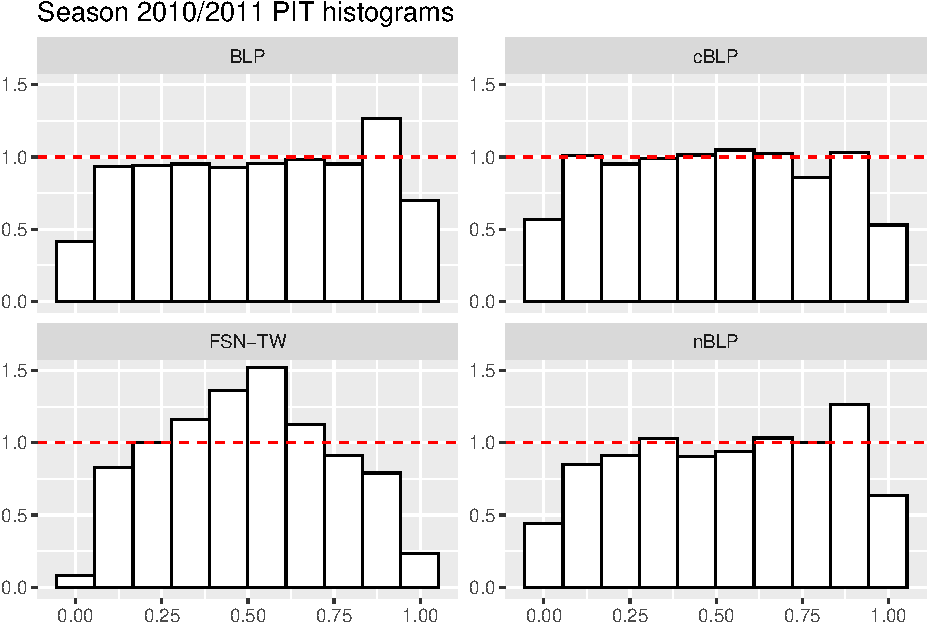
\includegraphics{applied_blp_sim_files/figure-latex/unnamed-chunk-5-1} 

}

\caption{Train PITs}\label{fig:unnamed-chunk-5}
\end{figure}

\clearpage

\begin{figure}[h]

{\centering 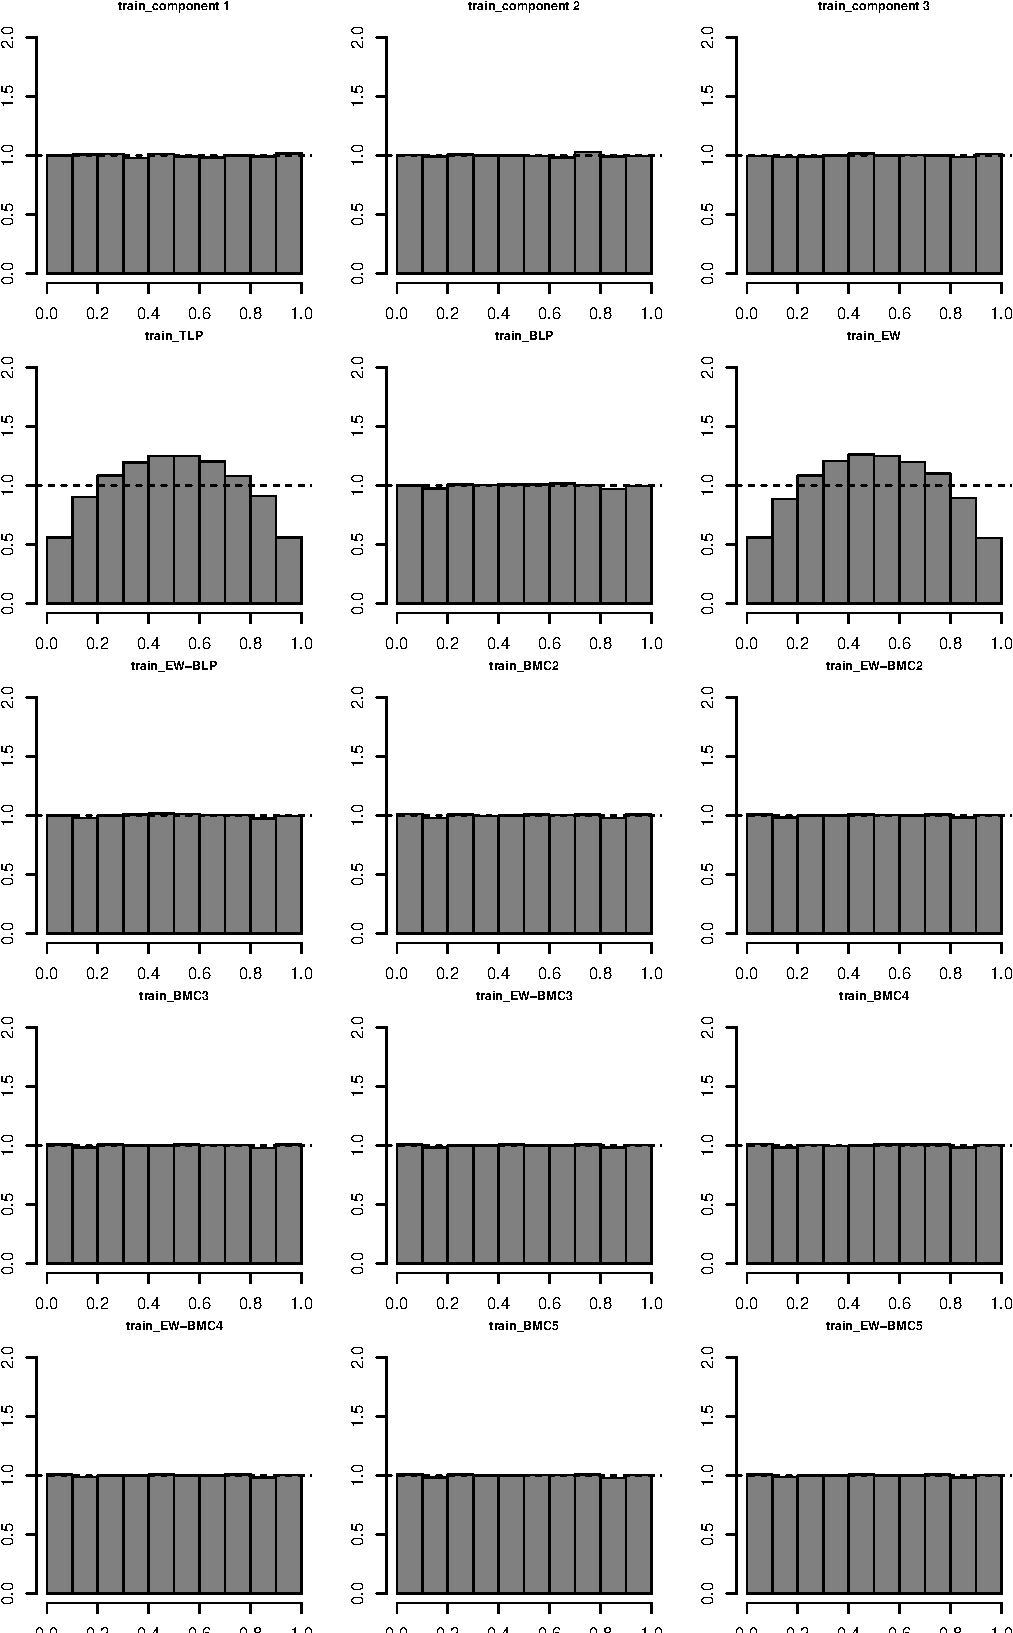
\includegraphics{applied_blp_sim_files/figure-latex/unnamed-chunk-6-1} 

}

\caption{Test PITs}\label{fig:unnamed-chunk-6}
\end{figure}

\clearpage

\hypertarget{scenario-2-multimodal-dgp-normal-mixture-and-close-mathcalm}{%
\subsection{\texorpdfstring{Scenario 2: Multimodal DGP (Normal mixture)
and
close-\(\mathcal{M}\)}{Scenario 2: Multimodal DGP (Normal mixture) and close-\textbackslash mathcal\{M\}}}\label{scenario-2-multimodal-dgp-normal-mixture-and-close-mathcalm}}

The data generating process for the observation \(y_t\) is

\[
y_t \overset{i.i.d.}{\sim} p_1\text{N}(-2,0.25)+p_2\text{N}(0,0.25)+p_3\text{N}(2,0.25), \\
t= 1,...,100,0000
\]

where \(p_1=0.2,p_2=0.2\), and \(p_3=0.6\). In this scenario, the three
component models are in the data generating process and the TLP's PITs
are approximately beta distributed (uniformly distributed,
specifically). This scenario serves to show the situation in which TLP
is an optimal method of combining forecast distributions. We expect BLP
and BMC to perform as equally well as TLP with higher complexity. In
other words, this is when BLP and BMC are not needed.

\begin{figure}[H]

{\centering 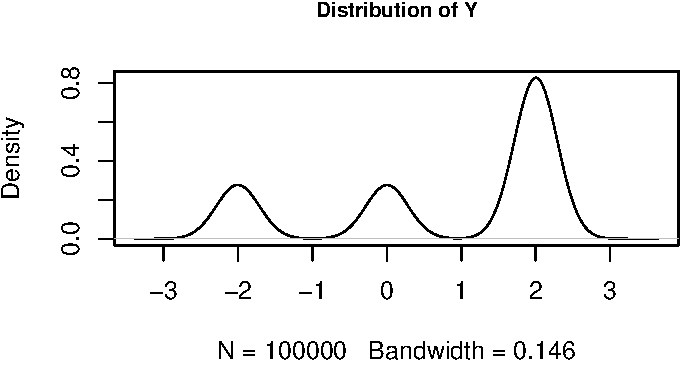
\includegraphics{applied_blp_sim_files/figure-latex/unnamed-chunk-8-1} 

}

\end{figure}

The individual predictive densities are defined as follows:

\[
\begin{aligned}
f_{1}&\overset{i.i.d.}{\sim}\text{N}(-2,0.25)\\
f_{2}&\overset{i.i.d.}{\sim}\text{N}(0,0.25)\\
f_{3}&\overset{i.i.d.}{\sim}\text{N}(2,0.25)\\
\end{aligned}
\]

\begin{table}[H]

\caption{\label{tab:unnamed-chunk-11}Cross validation log scores for beta mixture methods}
\centering
\fontsize{8}{10}\selectfont
\begin{tabular}[t]{l|r|r}
\hline
method & mean\_train\_ls & mean\_valid\_ls\\
\hline
BMC2 & -0.9812800 & -0.9815715\\
\hline
EW\_BMC2 & -1.0016930 & -1.0018338\\
\hline
BMC3 & -0.9812788 & -0.9815771\\
\hline
EW\_BMC3 & -0.9970163 & -0.9969911\\
\hline
BMC4 & -0.9812728 & -0.9815954\\
\hline
EW\_BMC4 & -0.9966951 & -0.9972928\\
\hline
BMC5 & -0.9812703 & -0.9815867\\
\hline
EW\_BMC5 & -0.9875902 & -0.9875473\\
\hline
\end{tabular}
\end{table}

\begin{table}[H]

\caption{\label{tab:unnamed-chunk-11}Weight Parameters}
\centering
\fontsize{8}{10}\selectfont
\begin{tabular}[t]{lrrrrr}
\toprule{}
Method & $w_1$ & $w_2$ & $w_3$ & $w_4$ & $w_5$\\
\midrule{}
TLP & NA & NA & NA & NA & NA\\
BLP & NA & NA & NA & NA & NA\\
EW & NA & NA & NA & NA & NA\\
EW-BLP & NA & NA & NA & NA & NA\\
BMC2 & 0.821 & 0.179 & NA & NA & NA\\
\addlinespace
EW-BMC5 & 0.317 & 0.014 & 0.229 & 0.221 & 0.219\\
\bottomrule{}
\end{tabular}
\end{table}

\begin{table}[H]

\caption{\label{tab:unnamed-chunk-11}Beta mixture parameters}
\centering
\fontsize{8}{10}\selectfont
\begin{tabular}[t]{lrrrrrrrrrr}
\toprule{}
Method & $\alpha_1$ & $\beta_1$ & $\alpha_2$ & $\beta_2$ & $\alpha_3$ & $\beta_3$ & $\alpha_4$ & $\beta_4$ & $\alpha_5$ & $\beta_5$\\
\midrule{}
TLP & NA & NA & NA & NA & NA & NA & NA & NA & NA & NA\\
BLP & 1.000 & 1.003 & NA & NA & NA & NA & NA & NA & NA & NA\\
EW & NA & NA & NA & NA & NA & NA & NA & NA & NA & NA\\
EW-BLP & 1.256 & 0.789 & NA & NA & NA & NA & NA & NA & NA & NA\\
BMC2 & 1.010 & 1.040 & 0.948 & 0.851 & NA & NA & NA & NA & NA & NA\\
\addlinespace
EW-BMC5 & 11.113 & 2.811 & 0.912 & 0.744 & 0.942 & 0.745 & 0.944 & 0.745 & 0.943 & 0.745\\
\bottomrule{}
\end{tabular}
\end{table}

\begin{table}[H]

\caption{\label{tab:unnamed-chunk-11}Component weight parameters -}
\centering
\fontsize{8}{10}\selectfont
\begin{tabular}[t]{lrrrrrrrrrrrrrrr}
\toprule{}
Method & $\omega_{11}$ & $\omega_{12}$ & $\omega_{13}$ & $\omega_{21}$ & $\omega_{22}$ & $\omega_{23}$ & $\omega_{31}$ & $\omega_{32}$ & $\omega_{33}$ & $\omega_{41}$ & $\omega_{42}$ & $\omega_{43}$ & $\omega_{51}$ & $\omega_{52}$ & $\omega_{53}$\\
\midrule{}
TLP & 0.198 & 0.200 & 0.602 & NA & NA & NA & NA & NA & NA & NA & NA & NA & NA & NA & NA\\
BLP & 0.197 & 0.200 & 0.603 & NA & NA & NA & NA & NA & NA & NA & NA & NA & NA & NA & NA\\
EW & 0.333 & 0.333 & 0.333 & NA & NA & NA & NA & NA & NA & NA & NA & NA & NA & NA & NA\\
EW-BLP & 0.333 & 0.333 & 0.333 & NA & NA & NA & NA & NA & NA & NA & NA & NA & NA & NA & NA\\
BMC2 & 0.212 & 0.166 & 0.622 & 0.121 & 0.369 & 0.510 & NA & NA & NA & NA & NA & NA & NA & NA & NA\\
\addlinespace
EW-BMC5 & 0.333 & 0.333 & 0.333 & 0.333 & 0.333 & 0.333 & 0.333 & 0.333 & 0.333 & 0.333 & 0.333 & 0.333 & 0.333 & 0.333 & 0.333\\
\bottomrule{}
\end{tabular}
\end{table}

\begin{table}[H]
\caption{\label{tab:unnamed-chunk-11}Log score}

\centering
\fontsize{8}{10}\selectfont
\begin{tabular}[t]{lrrrrrr}
\toprule{}
  & TLP & BLP & EW & EW-BLP & BMC2 & EW-BMC5\\
\midrule{}
Training & -0.981 & -0.981 & -1.132 & -1.043 & -0.981 & -0.999\\
Test & -0.991 & -0.991 & -1.139 & -1.053 & -0.991 & -1.011\\
\bottomrule{}
\end{tabular}
\end{table}

\clearpage

\begin{figure}[h]

{\centering 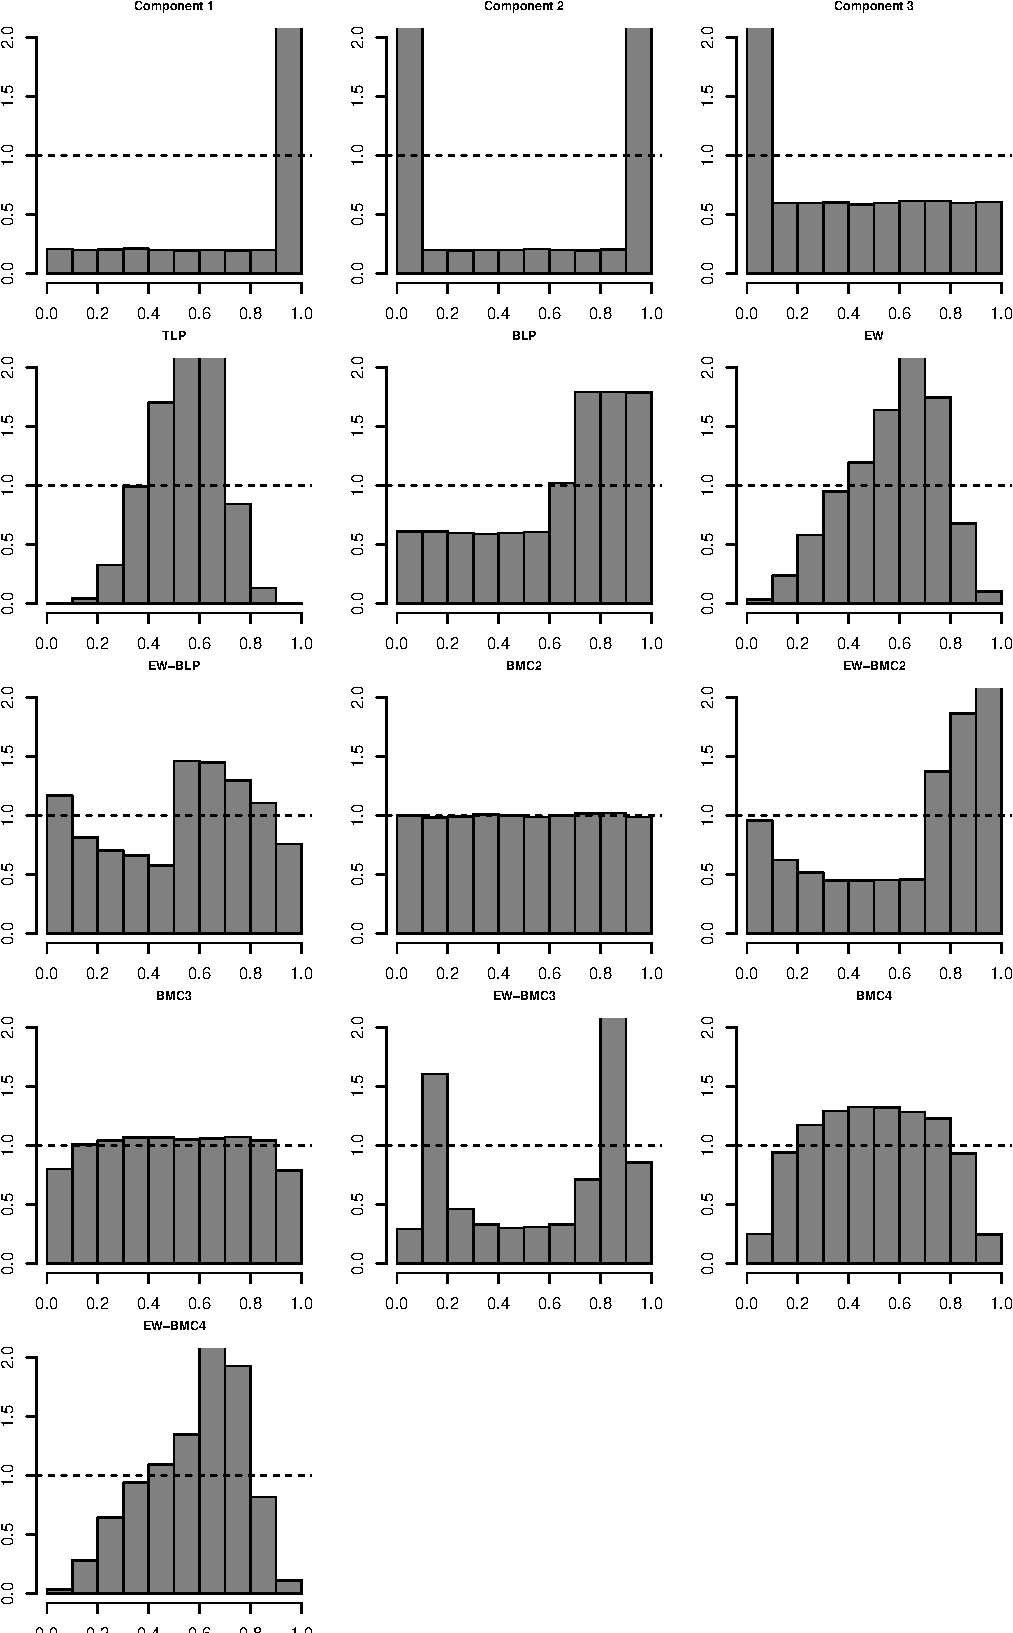
\includegraphics{applied_blp_sim_files/figure-latex/unnamed-chunk-12-1} 

}

\caption{Train PITs}\label{fig:unnamed-chunk-12}
\end{figure}

\clearpage

\begin{figure}[h]

{\centering 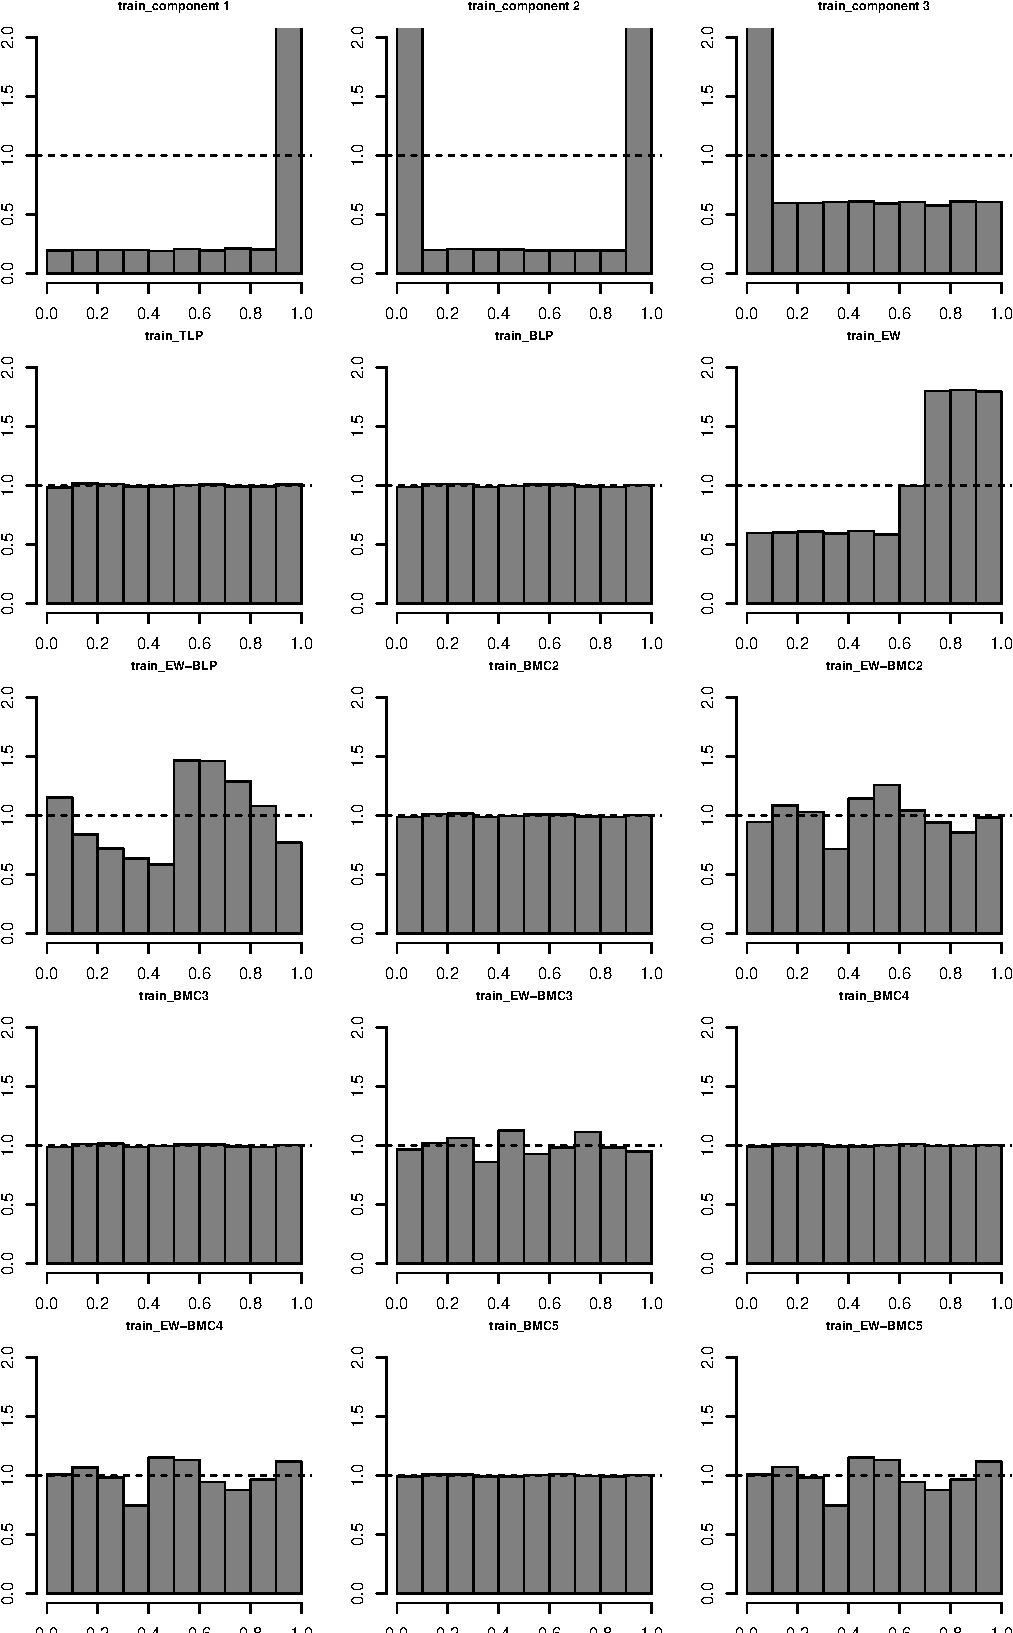
\includegraphics{applied_blp_sim_files/figure-latex/unnamed-chunk-13-1} 

}

\caption{Test PITs}\label{fig:unnamed-chunk-13}
\end{figure}

\clearpage

\begin{figure}[h]

{\centering 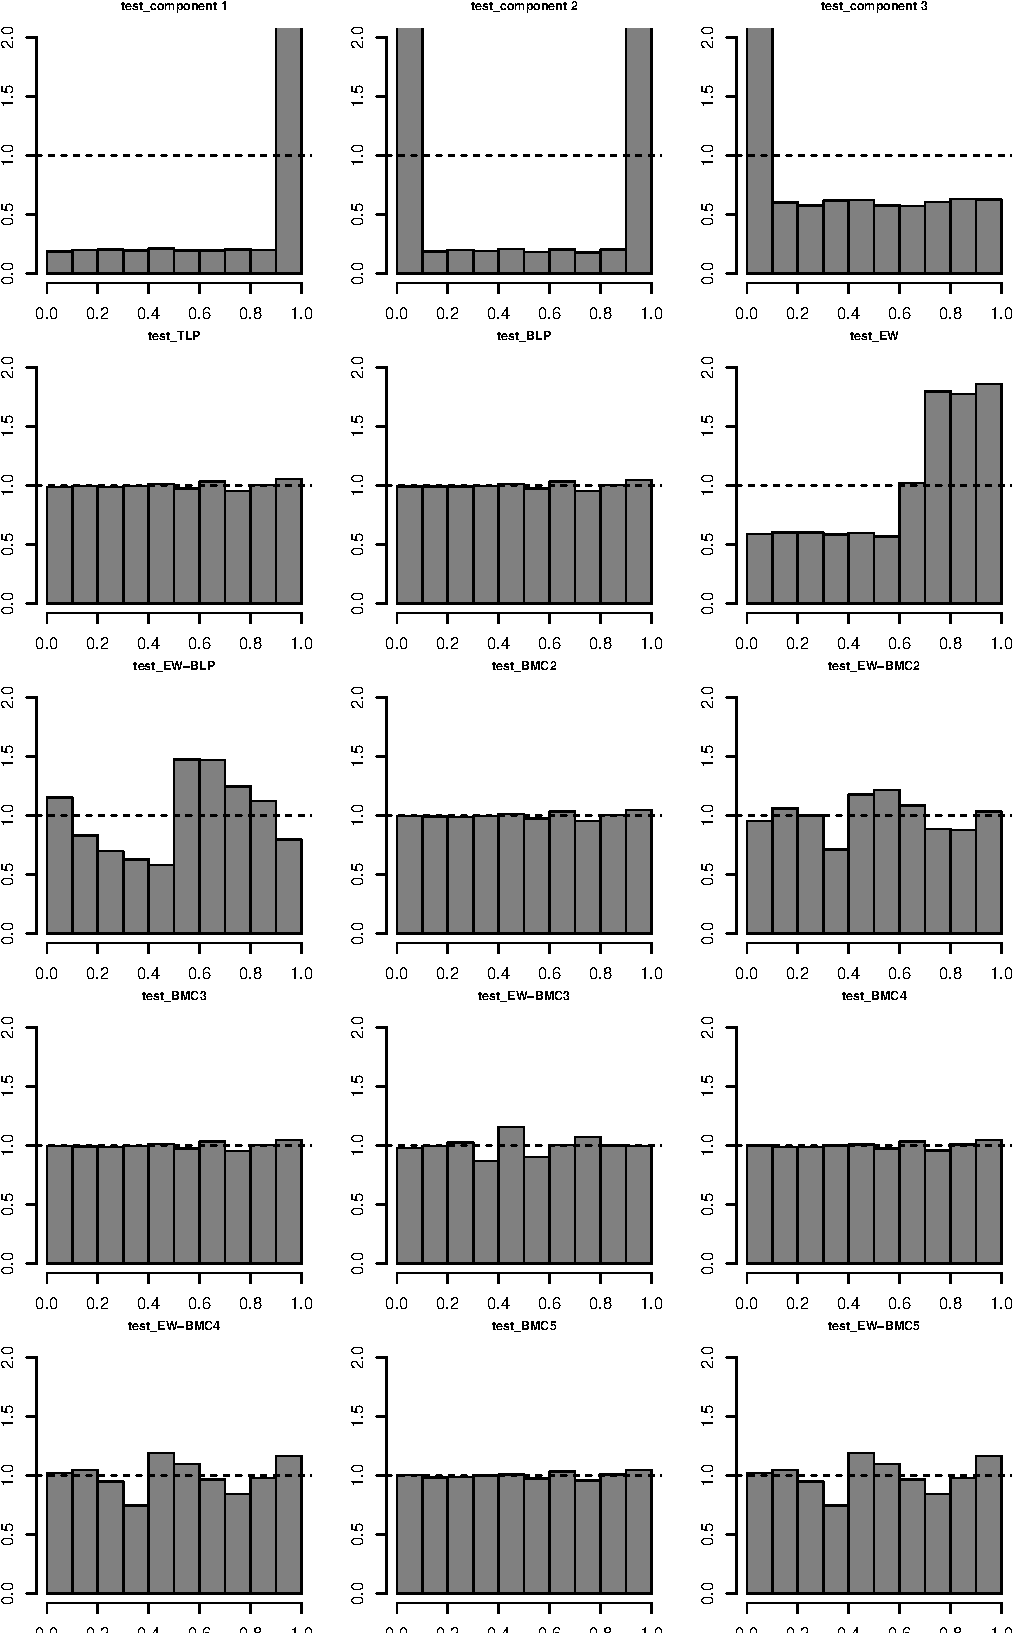
\includegraphics{applied_blp_sim_files/figure-latex/unnamed-chunk-14-1} 

}

\end{figure}

\clearpage

\begin{figure}[h]

{\centering 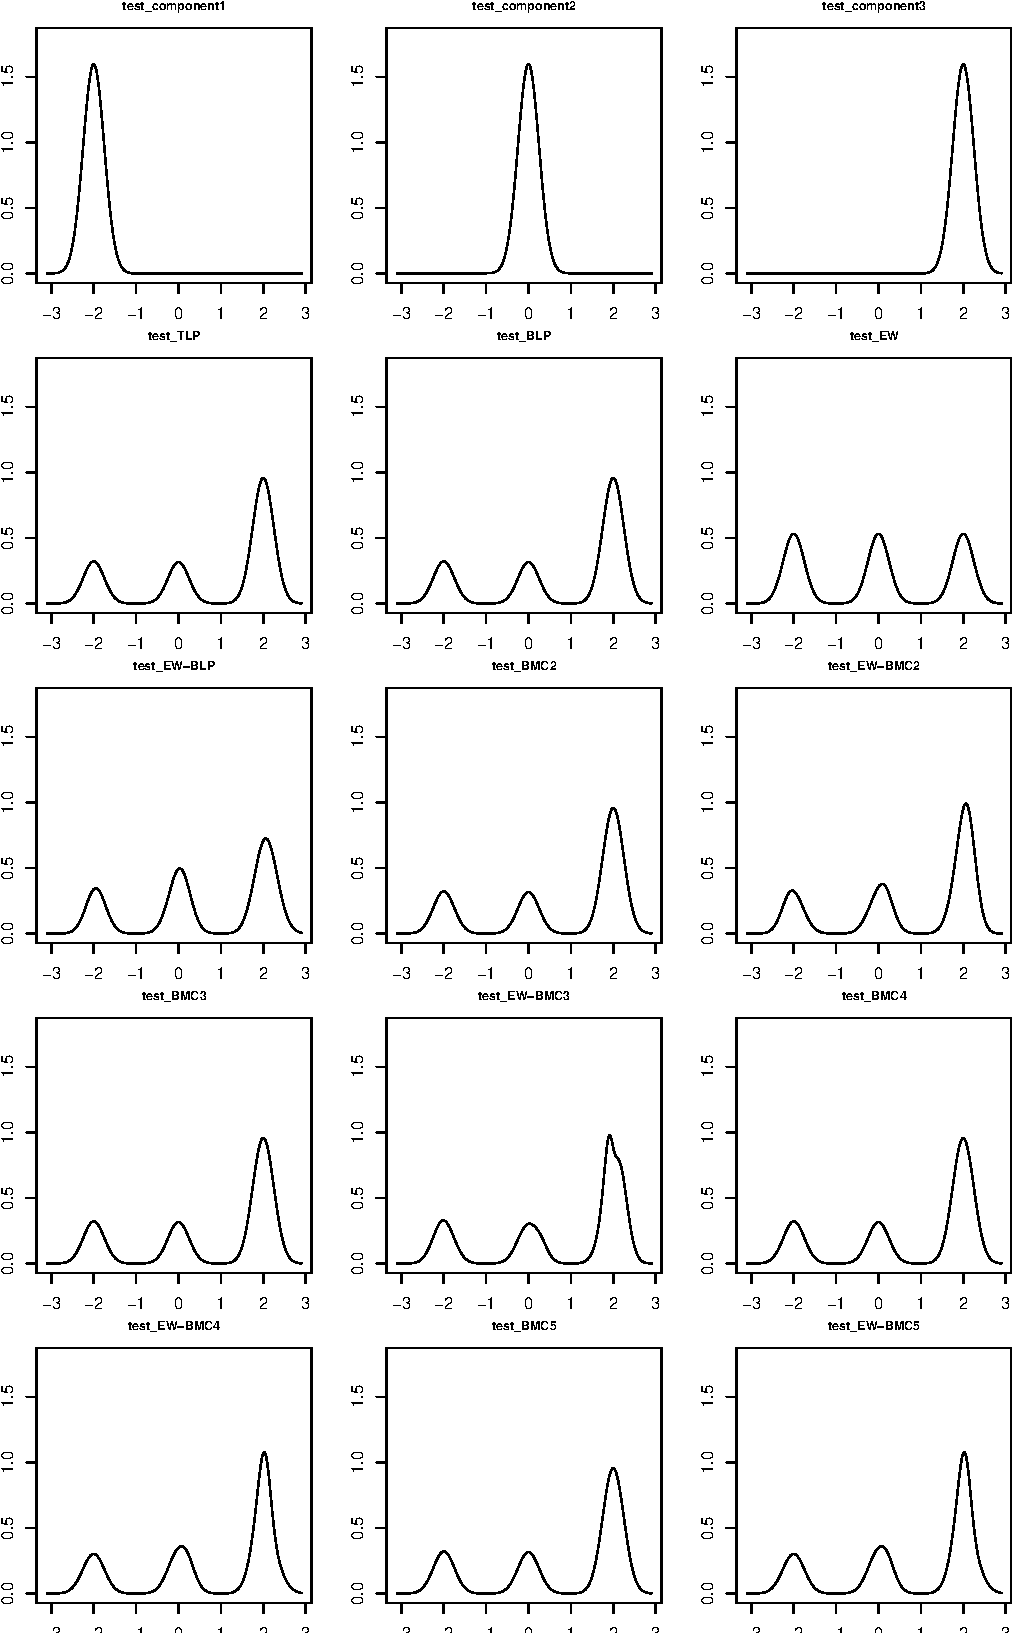
\includegraphics{applied_blp_sim_files/figure-latex/unnamed-chunk-15-1} 

}

\caption{Ensemble details}\label{fig:unnamed-chunk-15}
\end{figure}
\clearpage

\begin{figure}[h]

{\centering 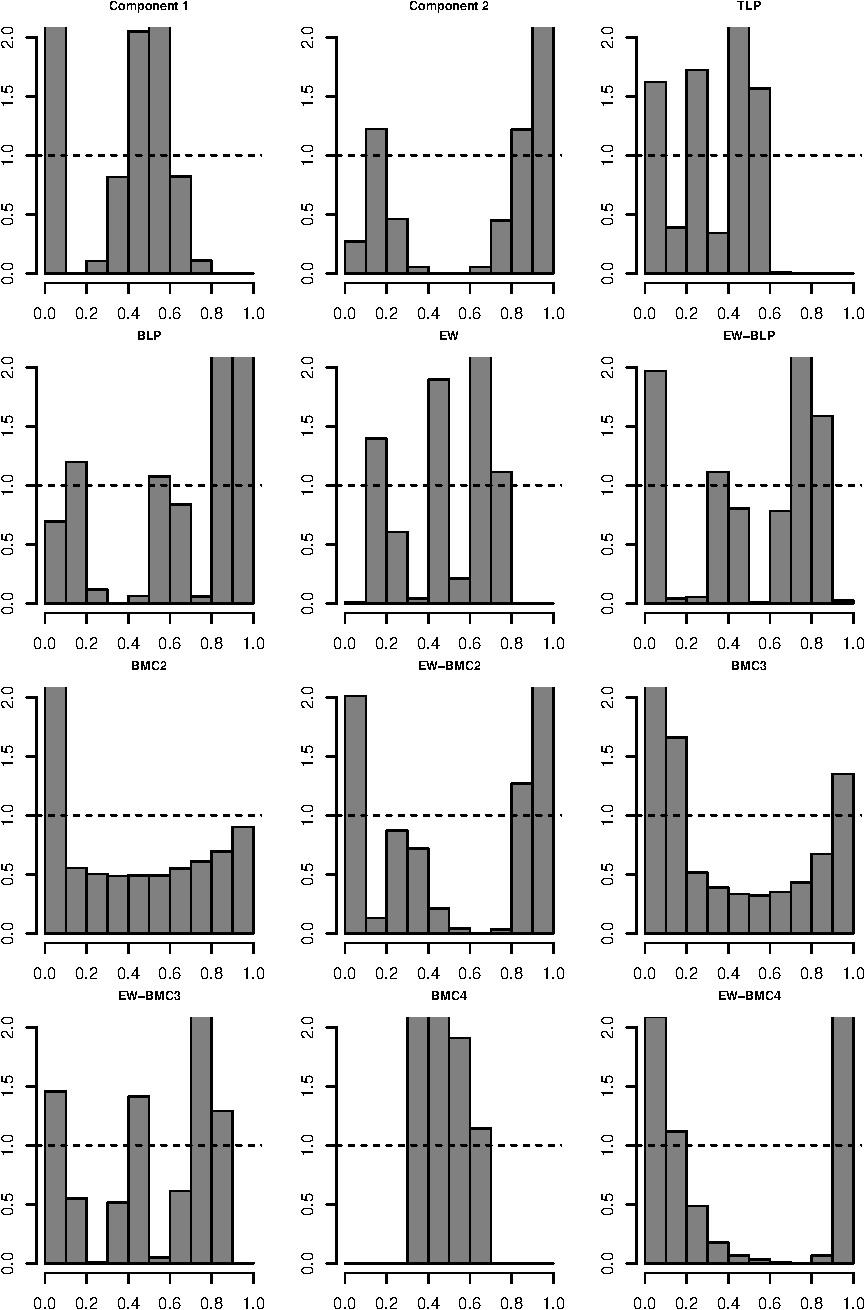
\includegraphics{applied_blp_sim_files/figure-latex/unnamed-chunk-16-1} 

}

\caption{Ensemble details}\label{fig:unnamed-chunk-16}
\end{figure}
\clearpage

\hypertarget{scenario-2.1-multimodal-dgp-normal-mixture-with-empirical-distributions}{%
\subsubsection{Scenario 2.1: Multimodal DGP (Normal mixture) with
empirical
distributions}\label{scenario-2.1-multimodal-dgp-normal-mixture-with-empirical-distributions}}

Using the same data generating process as the continuous distribution
version, but with \(t=2000\) so it computes faster. Since we calculate
the binned probability exactly from normal distributions, binned
probabilities (empirical pdfs) are exactly the same for all \(t\) in
each component model.

\begin{table}[H]
\caption{\label{tab:unnamed-chunk-19}Cross validation log scores for beta mixture methods}

\centering
\fontsize{8}{10}\selectfont
\begin{tabular}[t]{l}
\hline
x\\
\hline
BMC3\\
\hline
EW\_BMC4\\
\hline
\end{tabular}
\centering
\begin{tabular}[t]{l|r|r}
\hline
method & mean\_train\_ls & mean\_valid\_ls\\
\hline
BMC2 & -3.792627 & -3.747251\\
\hline
EW\_BMC2 & -3.818782 & -3.772621\\
\hline
BMC3 & -3.792136 & -3.746503\\
\hline
EW\_BMC3 & -3.813448 & -3.769789\\
\hline
BMC4 & -3.789741 & -3.746363\\
\hline
EW\_BMC4 & -3.809776 & -3.766783\\
\hline
BMC5 & -3.789478 & -3.747252\\
\hline
EW\_BMC5 & -3.809634 & -3.767397\\
\hline
\end{tabular}
\end{table}

\begin{table}[H]

\caption{\label{tab:unnamed-chunk-19}Weight Parameters}
\centering
\fontsize{8}{10}\selectfont
\begin{tabular}[t]{lrrrr}
\toprule{}
Method & $w_1$ & $w_2$ & $w_3$ & $w_4$\\
\midrule{}
TLP & NA & NA & NA & NA\\
BLP & NA & NA & NA & NA\\
EW & NA & NA & NA & NA\\
EW-BLP & NA & NA & NA & NA\\
BMC3 & 0.141 & 0.276 & 0.583 & NA\\
\addlinespace
EW-BMC4 & 0.075 & 0.080 & 0.615 & 0.23\\
\bottomrule{}
\end{tabular}
\end{table}

\begin{table}[H]

\caption{\label{tab:unnamed-chunk-19}Beta mixture parameters}
\centering
\fontsize{8}{10}\selectfont
\begin{tabular}[t]{lrrrrrrrr}
\toprule{}
Method & $\alpha_1$ & $\beta_1$ & $\alpha_2$ & $\beta_2$ & $\alpha_3$ & $\beta_3$ & $\alpha_4$ & $\beta_4$\\
\midrule{}
TLP & NA & NA & NA & NA & NA & NA & NA & NA\\
BLP & 0.506 & 2.008 & NA & NA & NA & NA & NA & NA\\
EW & NA & NA & NA & NA & NA & NA & NA & NA\\
EW-BLP & 0.607 & 2.035 & NA & NA & NA & NA & NA & NA\\
BMC3 & 0.083 & 13.274 & 0.725 & 3.993 & 0.487 & 5.330 & NA & NA\\
\addlinespace
EW-BMC4 & 0.968 & 64.938 & 0.082 & 14.852 & 0.773 & 9.565 & 0.315 & 11.957\\
\bottomrule{}
\end{tabular}
\end{table}

\begin{table}[H]

\caption{\label{tab:unnamed-chunk-19}Component weight parameters -}
\centering
\fontsize{8}{10}\selectfont
\begin{tabular}[t]{lrrrrrrrrrrrr}
\toprule{}
Method & $\omega_{11}$ & $\omega_{12}$ & $\omega_{13}$ & $\omega_{21}$ & $\omega_{22}$ & $\omega_{23}$ & $\omega_{31}$ & $\omega_{32}$ & $\omega_{33}$ & $\omega_{41}$ & $\omega_{42}$ & $\omega_{43}$\\
\midrule{}
TLP & 0.209 & 0.199 & 0.592 & NA & NA & NA & NA & NA & NA & NA & NA & NA\\
BLP & 0.216 & 0.200 & 0.584 & NA & NA & NA & NA & NA & NA & NA & NA & NA\\
EW & 0.333 & 0.333 & 0.333 & NA & NA & NA & NA & NA & NA & NA & NA & NA\\
EW-BLP & 0.333 & 0.333 & 0.333 & NA & NA & NA & NA & NA & NA & NA & NA & NA\\
BMC3 & 0.157 & 0.809 & 0.034 & 0.001 & 0.001 & 0.998 & 0.267 & 0.196 & 0.537 & NA & NA & NA\\
\addlinespace
EW-BMC4 & 0.333 & 0.333 & 0.333 & 0.333 & 0.333 & 0.333 & 0.333 & 0.333 & 0.333 & 0.333 & 0.333 & 0.333\\
\bottomrule{}
\end{tabular}
\end{table}

\begin{table}[H]
\caption{\label{tab:unnamed-chunk-19}Log score}

\centering
\fontsize{8}{10}\selectfont
\begin{tabular}[t]{lrrrrrr}
\toprule{}
  & TLP & BLP & EW & EW-BLP & BMC3 & EW-BMC4\\
\midrule{}
Training & -3.794 & -3.794 & -3.934 & -3.844 & -3.791 & -3.817\\
Test & -3.709 & -3.710 & -3.879 & -3.796 & -3.705 & -3.725\\
\bottomrule{}
\end{tabular}
\end{table}

\begin{figure}[h]

{\centering 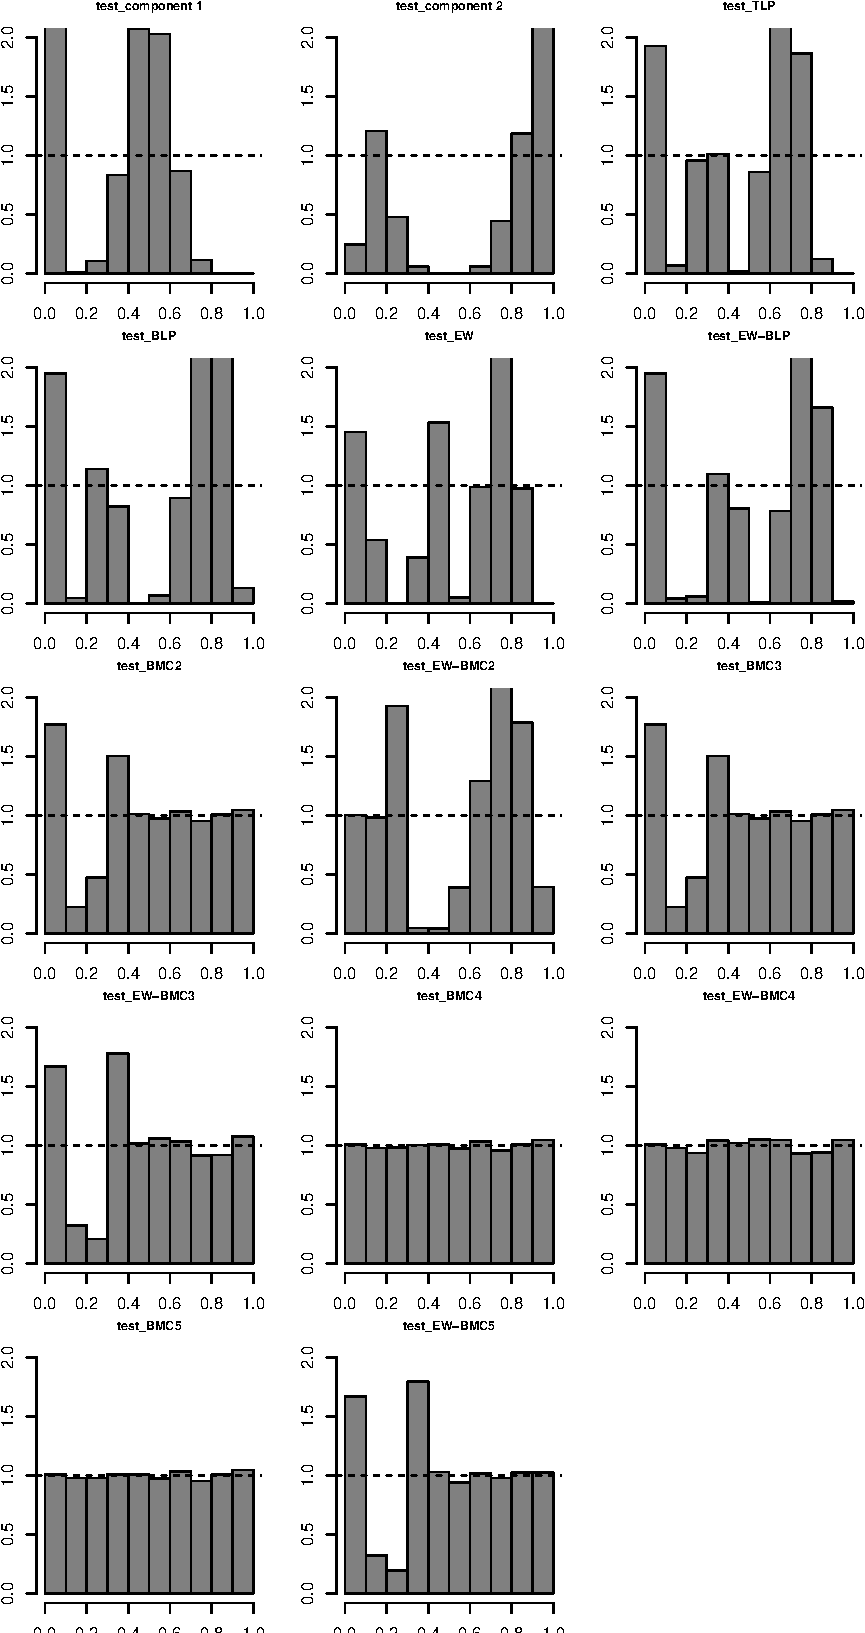
\includegraphics{applied_blp_sim_files/figure-latex/unnamed-chunk-20-1} 

}

\caption{Train PITs}\label{fig:unnamed-chunk-20}
\end{figure}

\clearpage

\begin{figure}[h]

{\centering 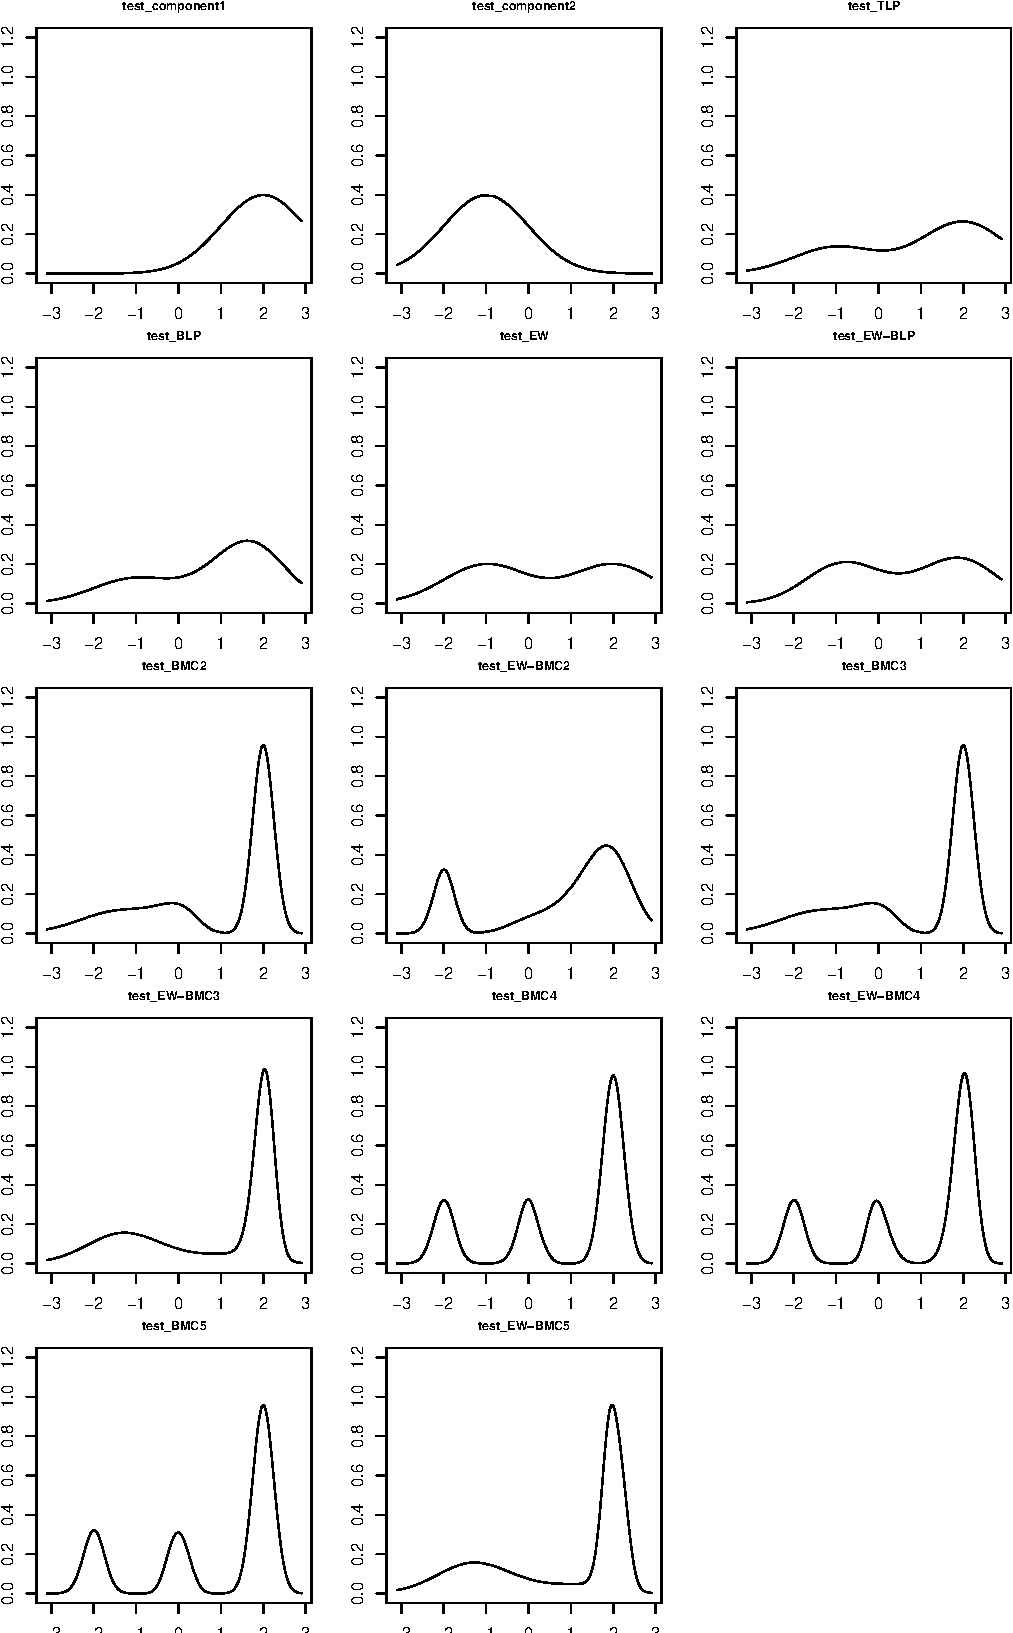
\includegraphics{applied_blp_sim_files/figure-latex/unnamed-chunk-21-1} 

}

\caption{Test PITs}\label{fig:unnamed-chunk-21}
\end{figure}
\clearpage

\hypertarget{scenario-3-misspecified-normal-mixture}{%
\subsection{Scenario 3: Misspecified Normal
mixture}\label{scenario-3-misspecified-normal-mixture}}

The data generating process for the observations in this scenario is the
same as in Scenario 2. There are two component models defined as follows

\[
\begin{aligned}
f_{1}&\overset{i.i.d.}{\sim}\text{N}(1.5,1)\\
f_{2}&\overset{i.i.d.}{\sim}\text{N}(0.5,1).\\
f_{3}&\overset{i.i.d.}{\sim}\text{N}(-2,1).\\
\end{aligned}
\]

The component models are not part of the data generating process. In
this scenario the TLP's PITs are not approximately beta distributed, so
we expect BLP to not be able to find optimal \(\alpha\) and \(\beta\) to
calibrate the PITs. Specifically, this scenario serves to motivate BMC
and show that BMC is highly flexible and can calibrate the PITs when BLP
cannot. We also expect BMC with higher K to be more flexible than BMC
with lower K.

\begin{table}[H]

\caption{\label{tab:unnamed-chunk-24}Cross validation log scores for beta mixture methods}
\centering
\fontsize{8}{10}\selectfont
\begin{tabular}[t]{l|r|r}
\hline
method & mean\_train\_ls & mean\_valid\_ls\\
\hline
BMC2 & -1.2073506 & -1.2066975\\
\hline
EW\_BMC2 & -1.2065485 & -1.2066941\\
\hline
BMC3 & -0.9742500 & -0.9746691\\
\hline
EW\_BMC3 & -1.1609765 & -1.1590791\\
\hline
BMC4 & -0.9745309 & -0.9748045\\
\hline
EW\_BMC4 & -1.0680773 & -1.0660947\\
\hline
BMC5 & -0.9746870 & -0.9751163\\
\hline
EW\_BMC5 & -0.9745933 & -0.9749492\\
\hline
\end{tabular}
\end{table}

\begin{table}[H]

\caption{\label{tab:unnamed-chunk-24}Weight Parameters}
\centering
\fontsize{8}{10}\selectfont
\begin{tabular}[t]{lrrrr}
\toprule{}
Method & $w_1$ & $w_2$ & $w_3$ & $w_4$\\
\midrule{}
TLP & NA & NA & NA & NA\\
BLP & NA & NA & NA & NA\\
EW & NA & NA & NA & NA\\
EW-BLP & NA & NA & NA & NA\\
BMC3 & 0.197 & 0.202 & 0.601 & NA\\
\addlinespace
EW-BMC4 & 0.057 & 0.197 & 0.202 & 0.544\\
\bottomrule{}
\end{tabular}
\end{table}

\begin{table}[H]

\caption{\label{tab:unnamed-chunk-24}Beta mixture parameters}
\centering
\fontsize{8}{10}\selectfont
\begin{tabular}[t]{lrrrrrrrr}
\toprule{}
Method & $\alpha_1$ & $\beta_1$ & $\alpha_2$ & $\beta_2$ & $\alpha_3$ & $\beta_3$ & $\alpha_4$ & $\beta_4$\\
\midrule{}
TLP & NA & NA & NA & NA & NA & NA & NA & NA\\
BLP & 2.162 & 1.320 & NA & NA & NA & NA & NA & NA\\
EW & NA & NA & NA & NA & NA & NA & NA & NA\\
EW-BLP & 1.557 & 0.910 & NA & NA & NA & NA & NA & NA\\
BMC3 & 13.202 & 13.356 & 4.356 & 55.587 & 19.529 & 8.880 & NA & NA\\
\addlinespace
EW-BMC4 & 75.832 & 15.237 & 20.262 & 99.713 & 56.823 & 68.511 & 65.866 & 9.36\\
\bottomrule{}
\end{tabular}
\end{table}

\begin{table}[H]

\caption{\label{tab:unnamed-chunk-24}Component weight parameters -}
\centering
\fontsize{8}{10}\selectfont
\begin{tabular}[t]{lrrrrrrrrrrr}
\toprule{}
Method & $\omega_{11}$ & $\omega_{12}$ & $\omega_{13}$ & $\omega_{21}$ & $\omega_{22}$ & $\omega_{23}$ & $\omega_{31}$ & $\omega_{32}$ & $\omega_{33}$ & $\omega_{41}$ & $\omega_{42}$\\
\midrule{}
TLP & 0.778 & 0.000 & 0.222 & NA & NA & NA & NA & NA & NA & NA & NA\\
BLP & 0.562 & 0.000 & 0.438 & NA & NA & NA & NA & NA & NA & NA & NA\\
EW & 0.333 & 0.333 & 0.333 & NA & NA & NA & NA & NA & NA & NA & NA\\
EW-BLP & 0.500 & 0.500 & NA & NA & NA & NA & NA & NA & NA & NA & NA\\
BMC3 & 0.003 & 0.000 & 0.997 & 1.0 & 0.0 & 0 & 0.998 & 0.0 & 0.002 & NA & NA\\
\addlinespace
EW-BMC4 & 0.500 & 0.500 & NA & 0.5 & 0.5 & NA & 0.500 & 0.5 & NA & 0.5 & 0.5\\
\bottomrule{}
\end{tabular}
\end{table}

\begin{table}[H]
\caption{\label{tab:unnamed-chunk-24}Log score}

\centering
\fontsize{8}{10}\selectfont
\begin{tabular}[t]{lrrrrrr}
\toprule{}
  & TLP & BLP & EW & EW-BLP & BMC3 & EW-BMC4\\
\midrule{}
Training & -1.718 & -1.657 & -1.857 & -1.742 & -0.975 & -0.977\\
Test & -1.722 & -1.660 & -1.858 & -1.747 & -0.993 & -0.994\\
\bottomrule{}
\end{tabular}
\end{table}

\clearpage

\begin{figure}[h]

{\centering \includegraphics{applied_blp_sim_files/figure-latex/unnamed-chunk-25-1} 

}

\caption{Train PITs}\label{fig:unnamed-chunk-25}
\end{figure}

\clearpage

\begin{figure}[h]

{\centering \includegraphics{applied_blp_sim_files/figure-latex/unnamed-chunk-26-1} 

}

\caption{Test PITs}\label{fig:unnamed-chunk-26}
\end{figure}

\clearpage

\begin{figure}[h]

{\centering \includegraphics{applied_blp_sim_files/figure-latex/unnamed-chunk-27-1} 

}

\end{figure}

\end{document}
